\documentclass[12pt,dvips]{report}
\setcounter{secnumdepth}{5}
\usepackage{epsfig}
%... include macros 
%differential operators
\newcommand{\grad}{\nabla}
\newcommand{\deld}{\nabla \cdot}
\newcommand{\lap}{\Delta}
%boldface in math mode
\newcommand{\bm}[1]{\mbox{{\boldmath ${#1}$}}}
% vectors and tensors
\renewcommand{\vec}[1]{{\bf #1}}
\newcommand{\gvec}[1]{\mbox{{\boldmath ${#1}$}}}
\newcommand{\ten}[1]{\bar{\bm{#1}}}
%derivatives
\newcommand{\od}[2]{\frac{d {#1}}{d {#2}}}
\newcommand{\ods}[2]{\frac{d^2{#1}}{d {{#2}^2}}}
\newcommand{\pd}[2]{\frac{\partial {#1}}{\partial {#2}}}
\newcommand{\pds}[2]{\frac{\partial^2{#1}}{\partial {{#2}^2}}}
\newcommand{\pdsm}[3]{\frac{\partial^2{#1}}{\partial {#2}\,\partial {#3}}}
%funtional analysis
\newcommand{\abs}[1]{\left| #1 \right|}
\newcommand{\norm}[1]{\left\| #1 \right\|}
\newcommand{\iprod}[2]{\left( #1, #2 \right)}
\newcommand{\dprod}[2]{\left\langle #1, #2 \right\rangle}
%real numbers
\newcommand{\field}[1]{\mathbb{#1}}
\newcommand{\R}{\field{R}}
%funciton spaces
\newcommand{\M}{\mathcal{M}}
%delimiters
\newcommand{\pl}{\left(}
\newcommand{\pr}{\right)}
\newcommand{\sbl}{\left[}
\newcommand{\sbr}{\right]}
\newcommand{\dbl}{\left[\hspace{-0.05cm}\left[}
\newcommand{\dbr}{\right]\hspace{-0.05cm}\right]}
\newcommand{\cbl}{\left\{ }
\newcommand{\cbr}{\right\} }
\newcommand{\eqn}[1]{equation \ref {eq:#1}} 
\newcommand{\Eqn}[1]{Equation \ref {eq:#1}} 
\newcommand{\eqnst}[2]{equations \ref{eq:#1} and \ref{eq:#2}} 
\newcommand{\Eqnst}[2]{Equations \ref{eq:#1} and \ref{eq:#2}} 
\newcommand{\eqns}[2]{equations \ref{eq:#1}--\ref{eq:#2}} 
\newcommand{\Eqns}[2]{Equations \ref{eq:#1}--\ref{eq:#2}}
\newcommand{\msection}[1]{ \vspace{.2in} {\noindent \bf #1}.}
\renewcommand{\for}{\mbox{for}\quad}
%\newcommand{\for}{\mbox{for}\quad}
\newcommand{\argmin}{\mbox{argmin}}
\newcommand{\argmax}{\mbox{argmax}}
\newcommand{\fig}[1]{figure \ref{fig:#1}} 
\newcommand{\Fig}[1]{Figure \ref{fig:#1}} 
\newcommand{\figst}[2]{figures \ref {fig:#1} and \ref {fig:#2}} 
\newcommand{\Figst}[2]{Figures \ref {fig:#1} and \ref {fig:#2}} 
\newcommand{\figs}[2]{figures \ref{fig:#1}--\ref{fig:#2}} 
\newcommand{\Figs}[2]{Figures \ref{fig:#1}--\ref{fig:#2}}
\newcommand{\tab}[1]{table \ref {tab:#1}} 
\newcommand{\Tab}[1]{Table \ref {tab:#1}} 
\newcommand{\tabst}[2]{tables \ref {tab:#1} and \ref {tab:#2}} 
\newcommand{\Tabst}[2]{Tables \ref {tab:#1} and \ref {tab:#2}} 
\newcommand{\tabs}[2]{tables \ref{tab:#1}--\ref{tab:#2}} 
\newcommand{\Tabs}[2]{Tables \ref{tab:#1}--\ref{tab:#2}}
\newtheorem{theorem}{Theorem}
\newenvironment{neqnarray}[1]{\begin{minipage}[t]{6.5in}  \begin{minipage}[b]{1.0in} #1 \end{minipage}  \begin{minipage}[b]{5.5in}\begin{eqnarray}}{\end{eqnarray}\end{minipage}\end{minipage}}
\newcommand{\bneqnarray}[2]{\\ \\ \fbox{\begin{neqnarray}{#1} #2 \end{neqnarray}}\\ \\ \noindent} 

\begin{document}           % End of preamble and beginning of text.
\begin{center} \bf Two-Phase Flow Formulation \end{center}

For a homogeneous medium and incompressible fluids, the equations
for two-phase flow in fractional flow form are
\begin{eqnarray}
\omega \pd{S_w}{t}  &=& - \deld \l[ \frac{k_{rn}}{\mu_n} f_w \pd{p_c}{S_w} \grad S_w - \frac{k_{rn}}{\mu_n} f_w (\rho_n - \rho_w) \vec g + f_w \vec q_t \r] \label{mass_balance}\\
\deld  \vec q_t &=& 0 \label{div_term} \\
\vec q_t &=& - K(S_w) \l[ \grad p_t  - \rho_t  \vec g \r] \\ 
K &=& \frac{k_{rw}}{\mu_w}+ \frac{k_{rn}}{\mu_w} \\
f_w &=& \frac{\frac{k_{rw}}{\mu_w}}{\frac{k_{rw}}{\mu_w}+ \frac{k_{rn}}{\mu_w}}\\
p_t &=& \frac{p_n + p_w}{2} + \int_{1}^{S_w}  (\frac{1}{2} - f_w(s)) \pd{p_c}{S_w}(s) ds \\
\rho_t &=& ((1-f_w)\rho_n + f_w \rho_w) 
\end{eqnarray}
in the unknowns $S_w$ and $p_t$.  The $p-s-k$ functions still have to
be specified, but we don't need their exact form in order to derive
the above equations from the standard two-phase formulation. I
included the set of equations above because there are so many
opportunities for sign errors. You should be able to plug all of the
equations into eqn \ref{mass_balance} and recover the equation for
the wetting phase in the standard two-phase approach. Note I've lumped the
intrinsic permeability into $k$ since the medium is homogeneous. Also,
$\vec g$ is the gravitational acceleration vector. In 1D, eqn
\ref{div_term} implies that $\vec q_t$ is a constant. So we'll just
consider it another parameter and solve the saturation equation (eqn \ref{mass_balance}) alone. Making this 1D (and incompressible) simplification and rearranging the
system above as an advection-diffusion equation we get
\begin{equation}
\omega \pd{S_w}{t}  = - \deld \l[ D(S_w) \grad S_w + F(S_w) \r]
\end{equation}
where the nonlinear diffusion coefficient $D$ and the advective flux function $F$ are given by
\begin{eqnarray}
D(S_w) &=& \frac{\frac{k_{rn}}{\mu_n} \frac{k_{rw}}{\mu_w}}{\frac{k_{rw}}{\mu_w}+ \frac{k_{rn}}{\mu_w}} \pd{p_c}{S_w}  \\
F(S_w) &=&  \frac{\frac{k_{rw}}{\mu_w}}{\frac{k_{rw}}{\mu_w}+ \frac{k_{rn}}{\mu_w}} \vec q_t - \frac{\frac{k_{rn}}{\mu_n} \frac{k_{rw}}{\mu_w}}{\frac{k_{rw}}{\mu_w}+ \frac{k_{rn}}{\mu_w}}  (\rho_n - \rho_w) \vec g
\end{eqnarray}
Now we specify the $p-s-k$ relations as the Van Genuchten-Mualem relations ($S_r < S_w \leq 1$):
\begin{eqnarray}
\bar{S} &=& \frac{S_w - S_r}{1 - S_r} \\
\bar{p}_c &=& \alpha p_c \\
\bar{p}_c &=& \( \bar{S}^{-1/m} - 1 \)^{1/n} \\
\od{\bar{p}_c}{\bar{S}} &=& \frac{-1}{nm}\( \bar{S}^{-1/m} - 1 \)^{1/n-1} \bar{S}^{-1/m-1} \\
k_{rw} &=& k_i \bar{S}^{1/2} \l[ 1-(1-\bar{S}^{1/m})^m \r]^2 \\
k_{rn} &=& k_i (1-\bar{S})^{1/2}(1-\bar{S}^{1/m})^{2m}
\end{eqnarray}
where $\alpha$ and $n$ are given and $m = 1 - 1/n$. Now given the
parameters $\rho_w$, $\rho_n$, $\alpha$, $n$, $\omega$, $\mu_n$,
$\mu_w$, and $k_i$ we can solve the saturation equations with suitable
boundary/initial conditions. I've included plots of $D$ and $F$ for
$n=1.5$ and some dummy parameters to show their shapes. $D$ is zero at
$S=1$ and $S=0$ even though you might think it blows up at $S=1$ from
looking at the formulation. $F$ is non-convex and non-monotone. $F$
becomes monotone in the absence of gravity. It looks like we will
probably have trouble in $D'$ and maybe also $F'$ as $S \rightarrow
1$, at least in the $1 < n < 2$ cases.


\begin{figure}
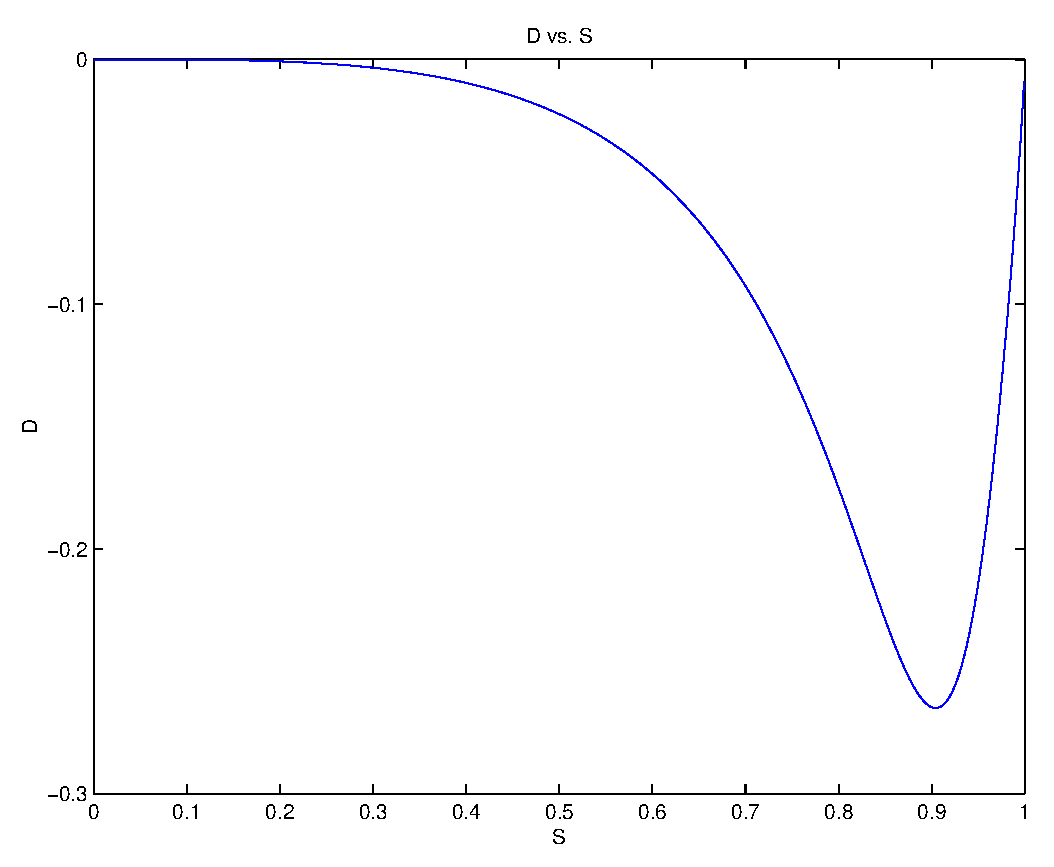
\epsfig{file=DvS.eps,scale=0.4} 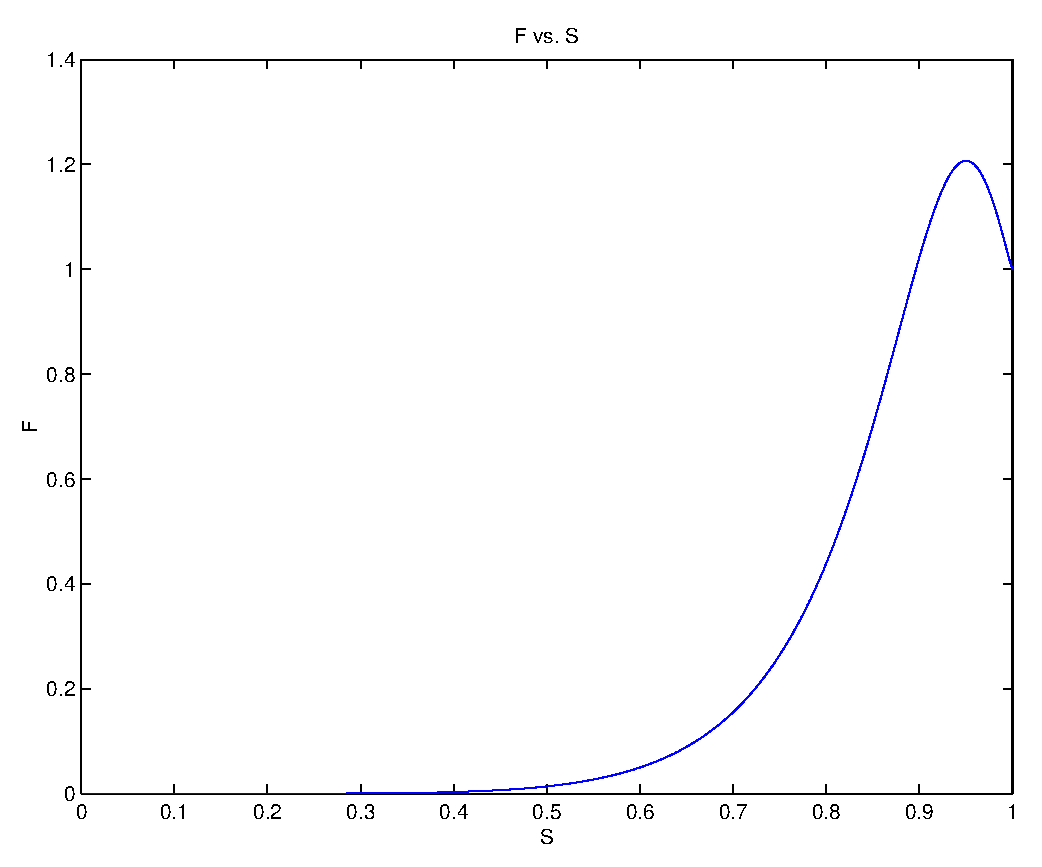
\epsfig{file=FvS.eps,scale=0.4}
\end{figure}
\newpage
A simple test problem on the horizontal domain $[0,1] \times [0,T]$
that has an analytical solution (McWhorter and Sunada) is based on the
boundary conditions
\begin{eqnarray}
S(0) &=& S_0 \\
S(1) &=& S_i \\
\end{eqnarray}
with the velocity field prescribed by 
\begin{equation}
q_t = A/\sqrt{t+t_0}
\end{equation}
and initial conditions
\begin{equation}
S(\vec x) = S^{*}(x,t_0)
\end{equation}
where $S^{*}$ is the analytical solution for the problem with the same
boundary conditions and the initial conditions $S^{*}(x,0) = S_i$. $A$
is a coefficient that is derived from the analytical solution. We take
the initial conditions for the test problem at the later time $t_0$ so
we avoid the problem of $A/\sqrt{t+t_0}$ being undefined. Figure
\ref{example1} shows plots of the analytical and numerical solutions
and the error for a 41 node cell-centered grid with upstream weighting
on the advective term and arithmetic averaging for $D$. Initial grid
refinement studies for this scheme shows first order convergence in
space on this problem in $L_1$ and $L_2$ while the convergence rate in
$L_{\infty}$ look like 0.7. The physical constants $t_0=0.1$, $T=0.4$,
$A \approx 0.111$, $g = 0$ , $\omega = 1$, $S_r = 0$, $ S_s = 1$,
$S_i=0.01$, $ S_0=0.9$, $n=4.264$, $k_i=1$, $\mu_w=1$, $\mu_n=1$, and
$\alpha=5.47$. To calculate the analytical solution using my matlab
functions first calculate the similarity solution by calling Fw(nn)
where nn is the number of spline knots.  1000 seems to be enough for
an accurate solution, but it can take a while. Right now there are
some divide by zero errors as well, but they don't seem to affect the
accuracy of the solution. Next initialize the solution at a particular
time, t, using initializeSw\_x(t). Thereafter Sw\_x(x) can be used to
evaluate $S^{*}(x,t)$ at points or vectors $x$.
\begin{figure}
\caption{Solutions (Top) Error (Bottom) \label{example1}}
\epsfig{file=example1Sol.eps,scale=0.7} 
\epsfig{file=example1Err.eps,scale=0.7}
\end{figure}
\end{document}









